\subsection{Autoencoders}
Autoencoders are networks that are trained to reconstruct their input. The usual architecture is something like
\cf{
\text{encoder} \to \text{bottleneck } h\to\text{decoder}
}
where the encoder encodes the input by some function into latent representation, and the decoder creates the reconstruction based on this representation. Architecture and regularization are chosen to preven simple copying. As the network learns by the discrepancy between input and reconstruction, autoencoders learn in an unsupervised fashion.

\subsection{Regularized Autoencoders}
\begin{itemize}
    \item Dimensionality \f{h \geq} dimensionality of \f{x \to} overcomplete representation
    \item Model capacity can be chosen based on the complexity of the data distribution.
    \item Prevent simple copying of the input e.g. by adding sparsity penalty on the hidden layer activations.
\end{itemize}

\subsection{Sparse Autoencoders}
\begin{itemize}
    \item Add a sparsity penalty \f{\Omega(h)} on the code \f{h} in the hidden layer to the loss function: \f{\fL + \Omega(h)}.
    \item Often used as an unsupervised pre-processing step for downstream supervised processing.
    \item Sparsity as regularization to avoid overfitting and increase generalization.
    \item Joint distribution: \f{p_{\text{model}}(x,h) = p_{\text{model}}(h)p_{\text{model}}(x|h)}
    \item We maximize: \f{\log p_{\text{model}}(x,h) = \log p_{\text{model}}(h)+\log p_{\text{model}}(x|h)}
    \item Sparsity can be implemented using a Laplace prior: \f{p_{\text{model}}(h_i) = \frac{\lambda}{2}\exp(-\lambda|h_i|),} where \f{\lambda} is a (learnable) hyperparameter
\end{itemize}

\subsection{Denoising Autoencoders}
Rather than adding an explicit regularization term, denoising autoencoders (DAE) learn to undo the effect of noise corruption when learning to reconstruct the input. To implement this, the input is corrupted by a corruption process \f{C(\tilde{x}|x)} before being fed into the encoder. The optimization is performed by the gradient descent with respect to the following negative log-likelihood. As a result, we obtain the reconstructed distribution \f{p(\tilde{x}|x)}. Note that the latent vector is deterministic in this method, but if we make it stochastic, it is equivalent to variational auto-encoder.


\subsection{\acp{vae}}
The idea behind generative models is to randomly sample from the latent space and decode to generate truly new data.\\
Assuming set of visible variables \f{x} and latent variables \f{z} our goal is to model the
distribution of the training data:
\cf{p(x)=\int p(x,z)dz = \int p(x|z)p(z)dz}
Once we have a good approximation of \f{p(x)}, we can sample from it and generate new
data that is very similar, but different from our original training data.\\

But how do we get \f{z} values that are related to our input data? This is the problem of inferring the posterior distribution \f{p(z|x)}. Since we can't use Bayes theorem to get \f{p(z|x)}, we have to resort to approximate inference methods:

\definition{Approximate inference methods approximate the posterior with a simpler distribution \f{q(z|x)} with its own set of parameters and optimize them to get as close as possible to \f{p(z|x)} by maximizing the evidence lower bound (ELBO), which minimizes the KL-Divergence.}

The \ac{vae} uses two neural networks: an encoder network with parameters \f{\phi} that learns to approximate the posterior \f{q_\phi(z|x)}, and a decoder network with parameters
\f{\theta} that learns to reconstruct the input \f{p_\theta(x|z)}. With this parametrization, the ELBO for variational inference is:
\cf{
    \fL(\theta, \phi, x) = - KL(q_\phi(z|x)\Vert p_\theta(z)) + \mathbb{E}_{q_\phi(z|x)}[\log p_\theta(x|z)]
}
where the first part is the regularization term and the second part is the reconstruction term.\\

To approximate the loss, we have to sample from posterior over \f{z}, but sampling is not a
continuous operation. To mitigate this, we can reparametrize to express our random variable \f{z} as a deterministic variable and an external, static noise source expressed in random variable \f{\epsilon}.

\begin{figure}[h!]
    \centering
    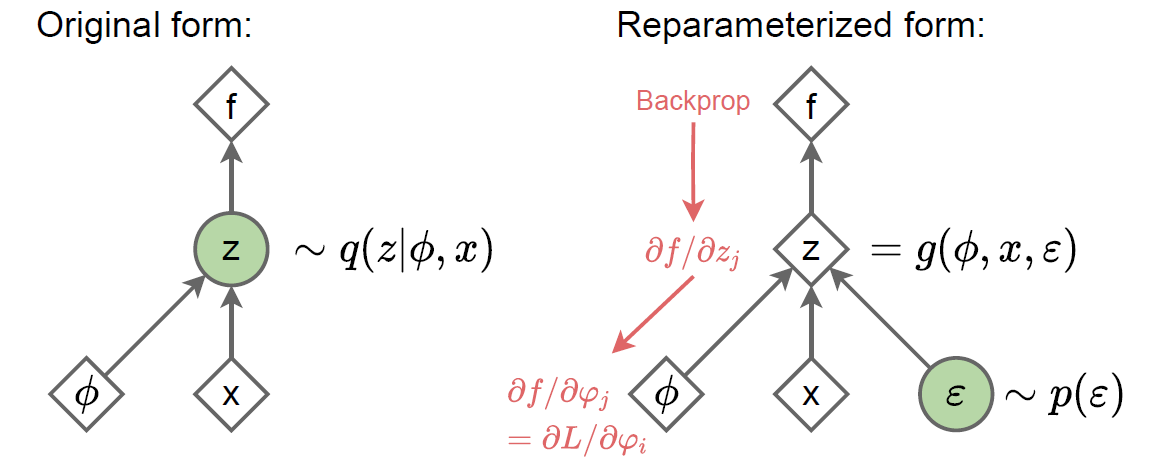
\includegraphics[width=0.6\textwidth]{reparam.png}
\end{figure}

With this reparametrization, both the decoder and the encoder can be trained together using backpropagation to optimize the ELBO.